\documentclass[presentation, 10pt]{beamer}
\usepackage{mystyle}
\addbibresource{committee_meeting_10_05_18_bib.bib}

\author{Scott Trinkle\newline \\
  Committee: Sam Armato, Tim Carroll, Sean Foxley, Patrick La Rivi\`ere}
\date{October 5, 2018}
\title{Committee Meeting: \\Validation of diffusion MRI
  with synchrotron x-ray micro-CT data}

\begin{document}

\frame{\titlepage}

\begin{frame}
  \frametitle{Outline}
  \begin{outline}
    \1 Background
    \2 Diffusion MRI
    \3 Reconstruction and validation
    \3 Tractography and validation
    \2 Synchrotron \uct
    
    \1 Potential aims
    \2 Aim 1: \uct acquisition and data processing optimization 
    \2 Aim 2: Validation of MRI ODFs with \uct data using structure tensor analysis
    \2 Aim 3: Validation of MRI tractography algorithms using \uct ODFs

    \1 Timeline
  \end{outline}
\end{frame}

\begin{frame}
  \frametitle{Diffusion MRI}
  \begin{outline}
    \1 Non-invasively estimates the bulk orientation-dependent diffusion within a voxel
    \1 Data reconstructed into an orientation distribution function (ODF)
    \2 3D profile of diffusion anisotropy
    \1 It is assumed that this ODF carries information about underlying tissue microstructure
  \end{outline}
\end{frame}

\begin{frame}
  \frametitle{Diffusion MRI: Reconstruction methods}
  \begin{figure}[h]
    \centering
    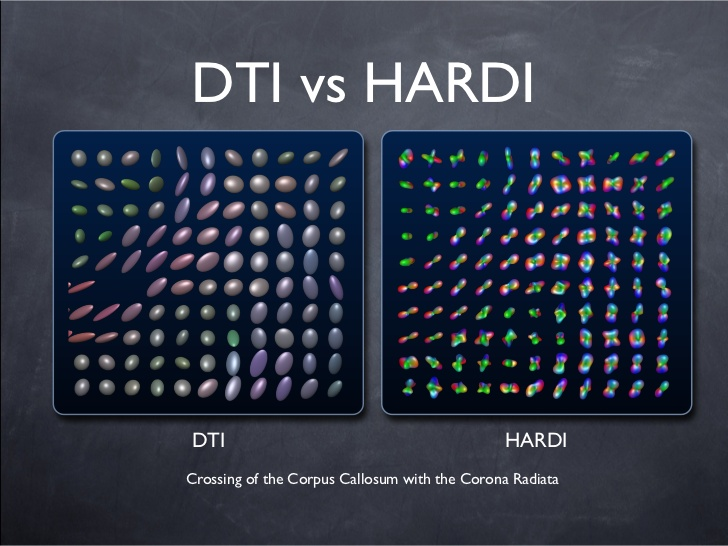
\includegraphics[width=0.7\textwidth]{figs/dtihardi}
    \label{fig:dtivshardi}
  \end{figure}
  \begin{center}
    \tiny{\href{https://www.slideshare.net/NFBI/bram-platel}{https://www.slideshare.net/NFBI/bram-platel}}
  \end{center}
\end{frame}

\begin{frame}
  \frametitle{Diffusion MRI: Previous reconstruction validation}
  \begin{outline}
    \1 Past groups have validated these ODF reconstructions using an image processing technique
    called ``structure tensor analysis''
    \2 Uses image gradients to estimate the direction of smallest intensity variation at each voxel\cite{Bigun1987}.
    \2 Bin these directions into a ground truth ODF

    \1 Most groups have used 2D histology images as ground truth\cite{Budde2012, Budde2013, Mitter2015, Seehaus2015}
    \2 Others have used polarized light imaging\cite{Mollink2017, Axer2016}, and 3D confocal stacks\cite{Schilling2016, Schilling2018, Khan2015}

    \1 \textbf{All previous validation datasets require physical sectioning of
      the sample and do not have isotropic resolution in 3D.}
    \2 This introduces a number of additional processing steps and sources of error in
    the validation pipeline.
  \end{outline}
\end{frame}

\begin{frame}
  \frametitle{Diffusion MRI: Previous reconstruction validation}
  \begin{columns}
    \begin{column}{0.7\textwidth}
      \begin{center}
        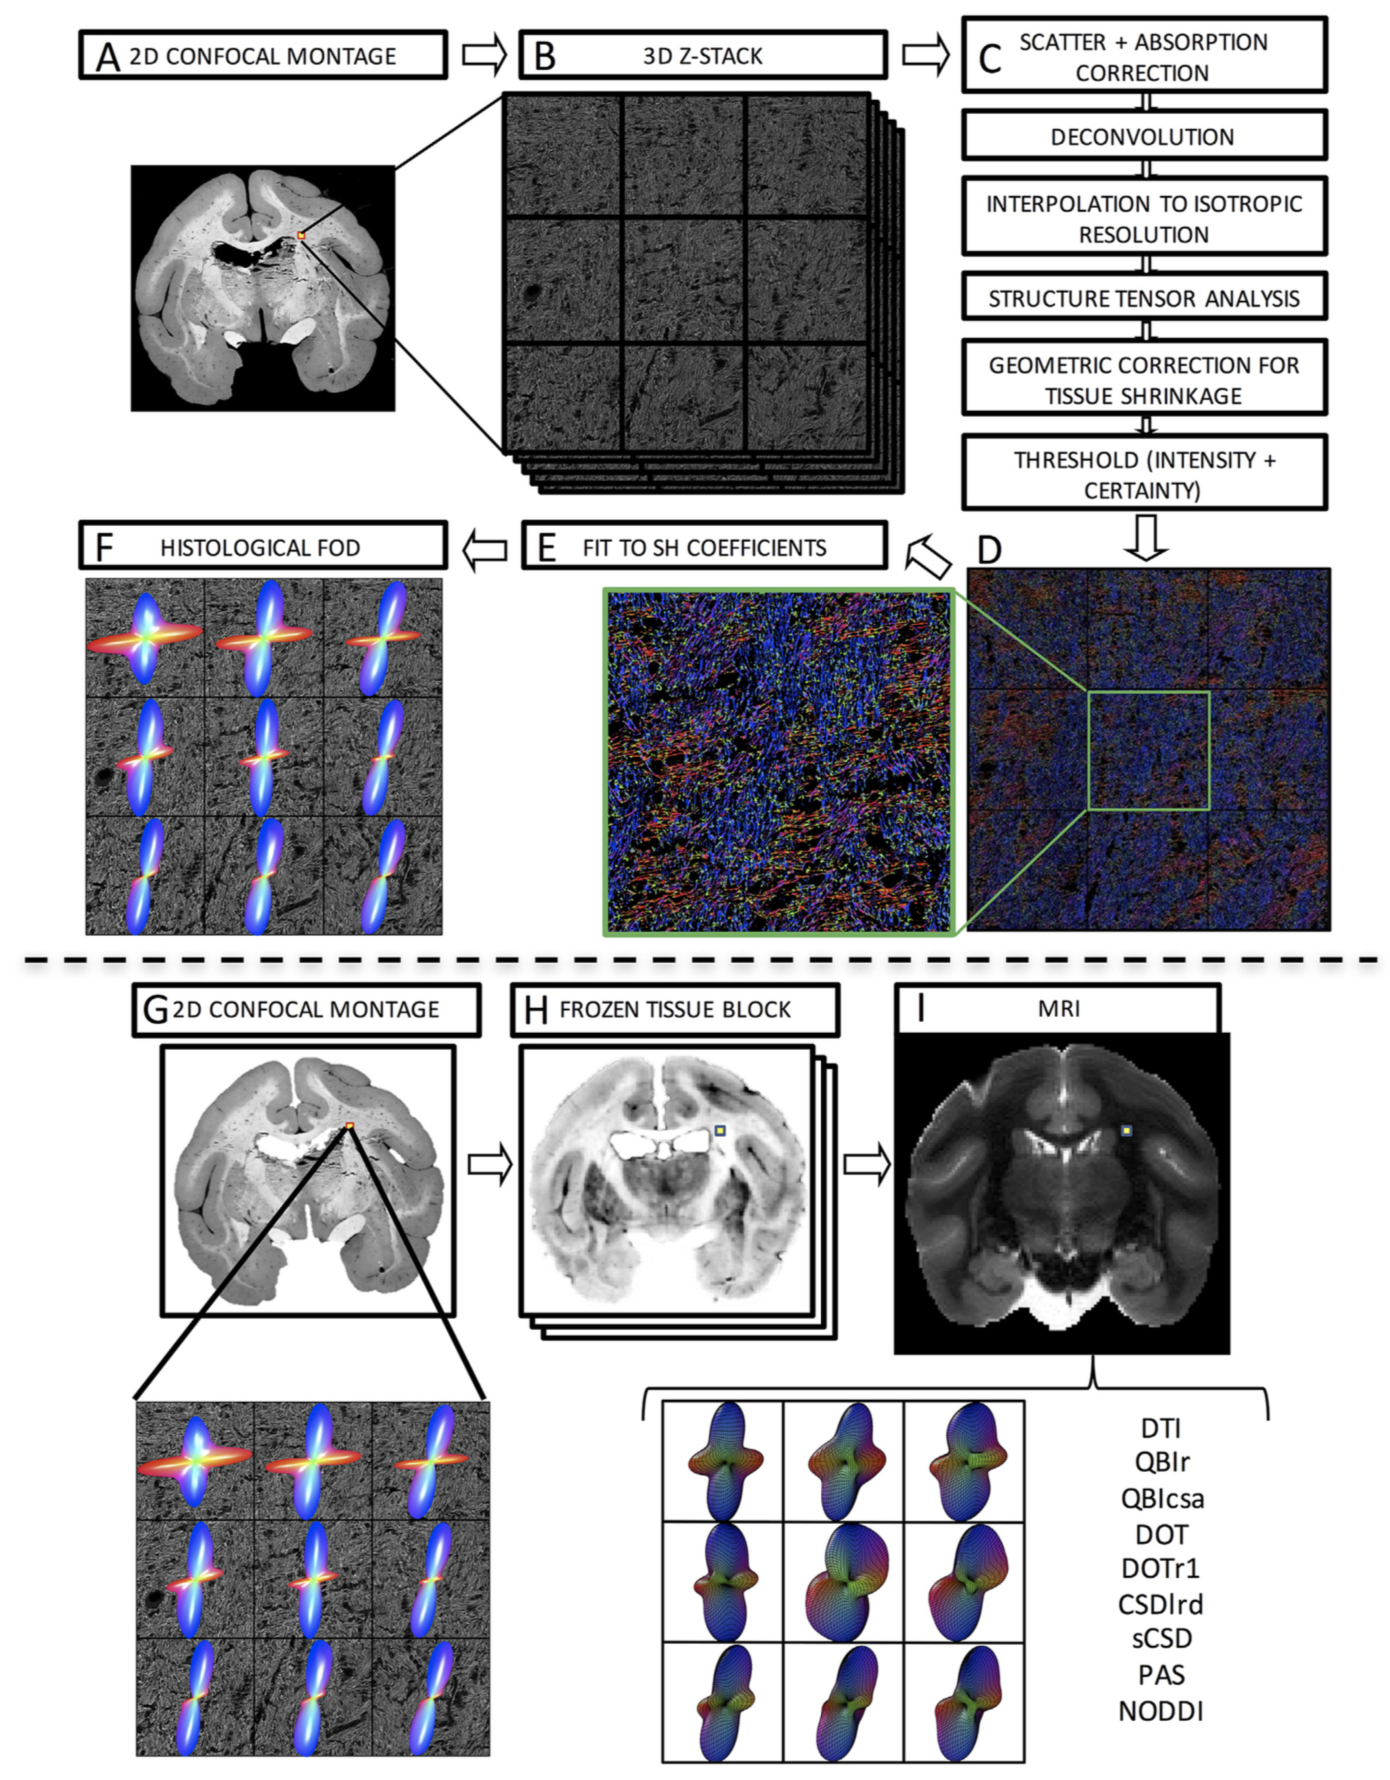
\includegraphics[height=0.9\textheight]{figs/schilling}
      \end{center}
    \end{column}
    \begin{column}{0.3\textwidth}
      \centering
      \small{Schilling 2018\cite{Schilling2018}}
    \end{column}    
  \end{columns}
\end{frame}

\begin{frame}
  \frametitle{Diffusion MRI: Tractography}

  \begin{figure}[h]
    \centering
    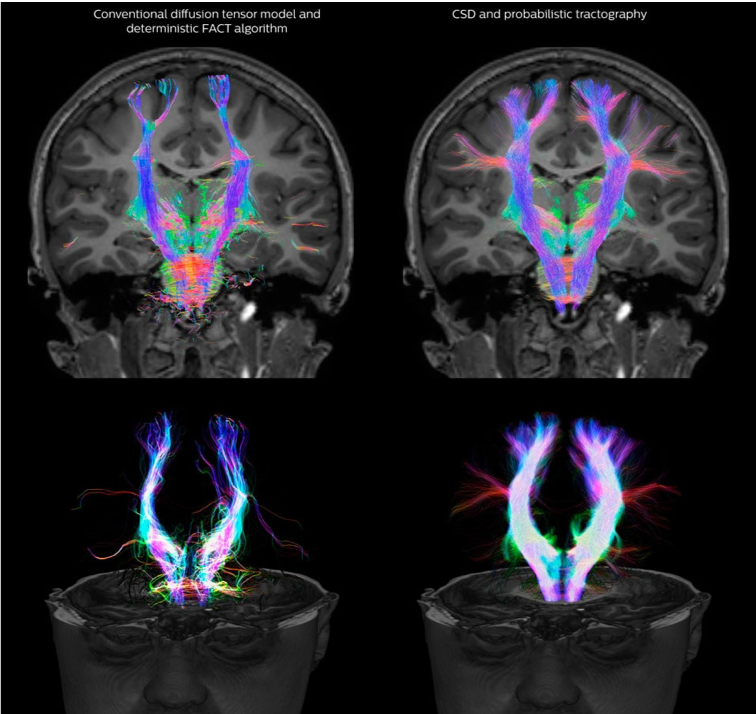
\includegraphics[width=0.65\textwidth]{figs/tractography}
    \label{fig:tractography}
  \end{figure}
  \begin{center}
    \tiny{\href{https://www.usa.philips.com/healthcare/education-resources/publications/fieldstrength/studying-connectivity-between-brain-regions}{https://www.usa.philips.com/healthcare/education-resources/publications/fieldstrength/studying-connectivity-between-brain-regions}}    
  \end{center}
\end{frame}

\begin{frame}
  \frametitle{Diffusion MRI: Previous tractography validation}
  \begin{outline}
    \1 Some groups have used synthetic data\cite{Maier-Hein2017}

    \1 Most groups have injected neural tract tracers, formed a
    3D histological volume and compared the fibers to tractography results using
    the injection sites as seeds.\cite{Donahue2016, Calabrese2015, Knosche2015, Thomas2014, Seehaus2013, Dauguet2007}
    \2 Non-isotropic resolution, requires physical sectioning
    \2 Limited to the number of tracer injection sites
    
    \1 General result is a dramatic sensitivity/specificity tradeoff

    \1 Again, \uct overcomes the limitations of histology as a validation
    dataset, and potentially allows for validation over the entire connectome.
  \end{outline}
\end{frame}

\begin{frame}
  \frametitle{Synchrotron \bolduct}
  \begin{center}
    \includemedia[
    width=9cm, height=5.8634cm,
    activate=pageopen,
    addresource=figs/recon_8x_04_18.mp4,
    flashvars={
      source=figs/recon_8x_04_18.mp4
    }
    ]{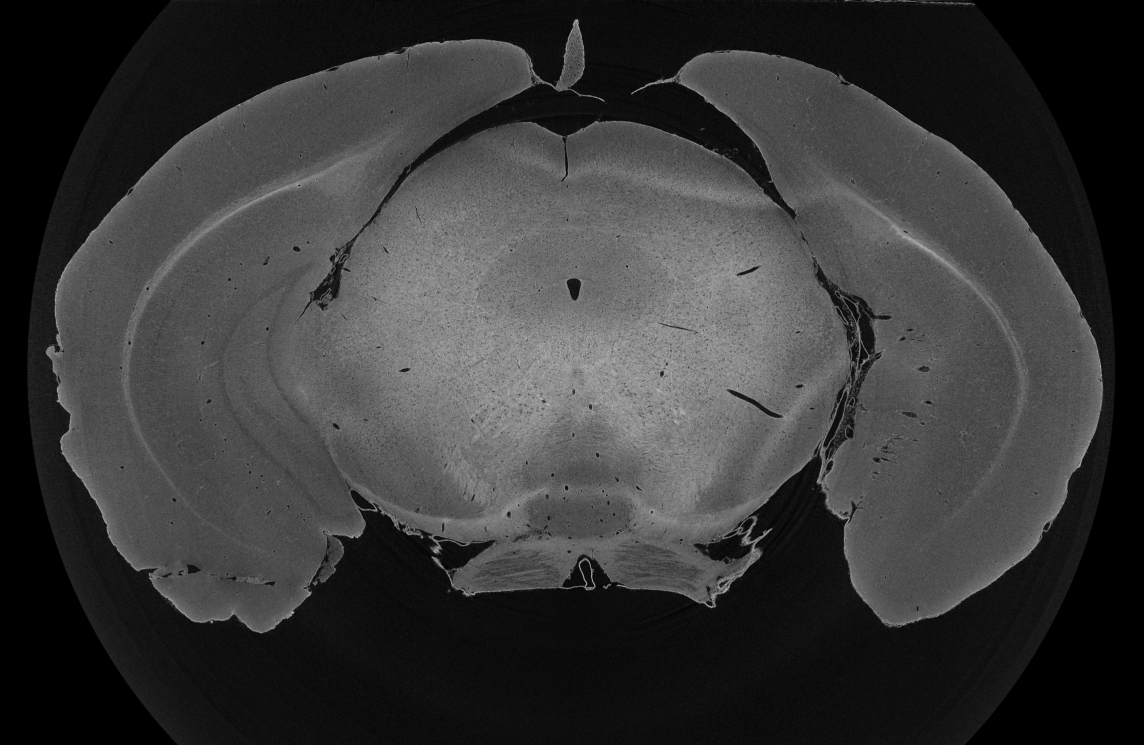
\includegraphics[width=9cm, height=5.8634cm]{figs/xrayvidposter}}{VPlayer9.swf}                    
  \end{center}
\end{frame}

\begin{frame}
  \frametitle{Data acquisition}
  \tikzstyle{block} = [rectangle, draw, fill=uclightgray, text centered, rounded corners, minimum height=1em, minimum width=1em]  
  \begin{center}
    \begin{tikzpicture}[scale=0.355]
      \scriptsize
      \node [block] (mriprep) at (0,0){
        \begin{tabular}{c}
          \textbf{Perfusion-fixed}\\
          \textbf{mouse brain}
        \end{tabular}
      };
      \node [block] (dmriacq) at (8, 0){\textbf{dMRI Acquisition}};
      \draw[->, double] (mriprep) to (dmriacq);
      \node (mrispecs) at (8, -3){
        \scriptsize{\begin{tabular}{c}
                      Bruker 9.4 T Magnet\\
                      150 $\upmu$m isotropic resolution\\
                      b-value: 3000 s/mm$^2$\\
                      30 uniformly distributed directions
                    \end{tabular}}        
      };
      \draw[-, double] (dmriacq) to (mrispecs);
      \node [block] (mrifods) at (8, -7){\textbf{dMRI ODFs}};
      \draw[->, double] (mrispecs) to (mrifods);
      \node [block] (xrayprep) at (16,0){\textbf{Sample staining}};
      \draw[->, double] (dmriacq) to (xrayprep);
      \node (stainnotes) at (16, -2.75){
        \scriptsize{\begin{tabular}{c}
                      uranyl acetate\\
                      osmium tetroxide\\
                      lead citrate\\
                    \end{tabular}}
      };
      \draw[-, double] (xrayprep) to (stainnotes);
      \node [block] (xrayacq) at (24, 0){\textbf{$\bm{\upmu}$CT Acquisition}};
      \draw[->, double] (xrayprep) to (xrayacq);
      \node (xrayspecs) at (24, -2.75){
        \scriptsize{\begin{tabular}{c}
                      APS at Argonne National Lab\\
                      Mosaic sinogram stitching \\
                      1.2 $\upmu$m isotropic resolution\\
                    \end{tabular}}
      };
      \draw[-, double] (xrayacq) to (xrayspecs);
      \node [block] (xrayfods) at (24, -7){\textbf{$\bm{\upmu}$CT ODFs}};
      \draw[->, double] (xrayspecs) to (xrayfods);
      \draw[<->, dashed] (mrifods) to (xrayfods);
      \node (compare) at (16, -7.5) {\scriptsize{Quantitative comparison}};

      \node [block] (em) at (30, 0){\textbf{EM}};
      \draw[->, double] (xrayacq) to (em);
    \end{tikzpicture}
  \end{center}
\end{frame}

\begin{frame}
  \frametitle{Data acquisition}
  \begin{figure}[h]
    \centering
    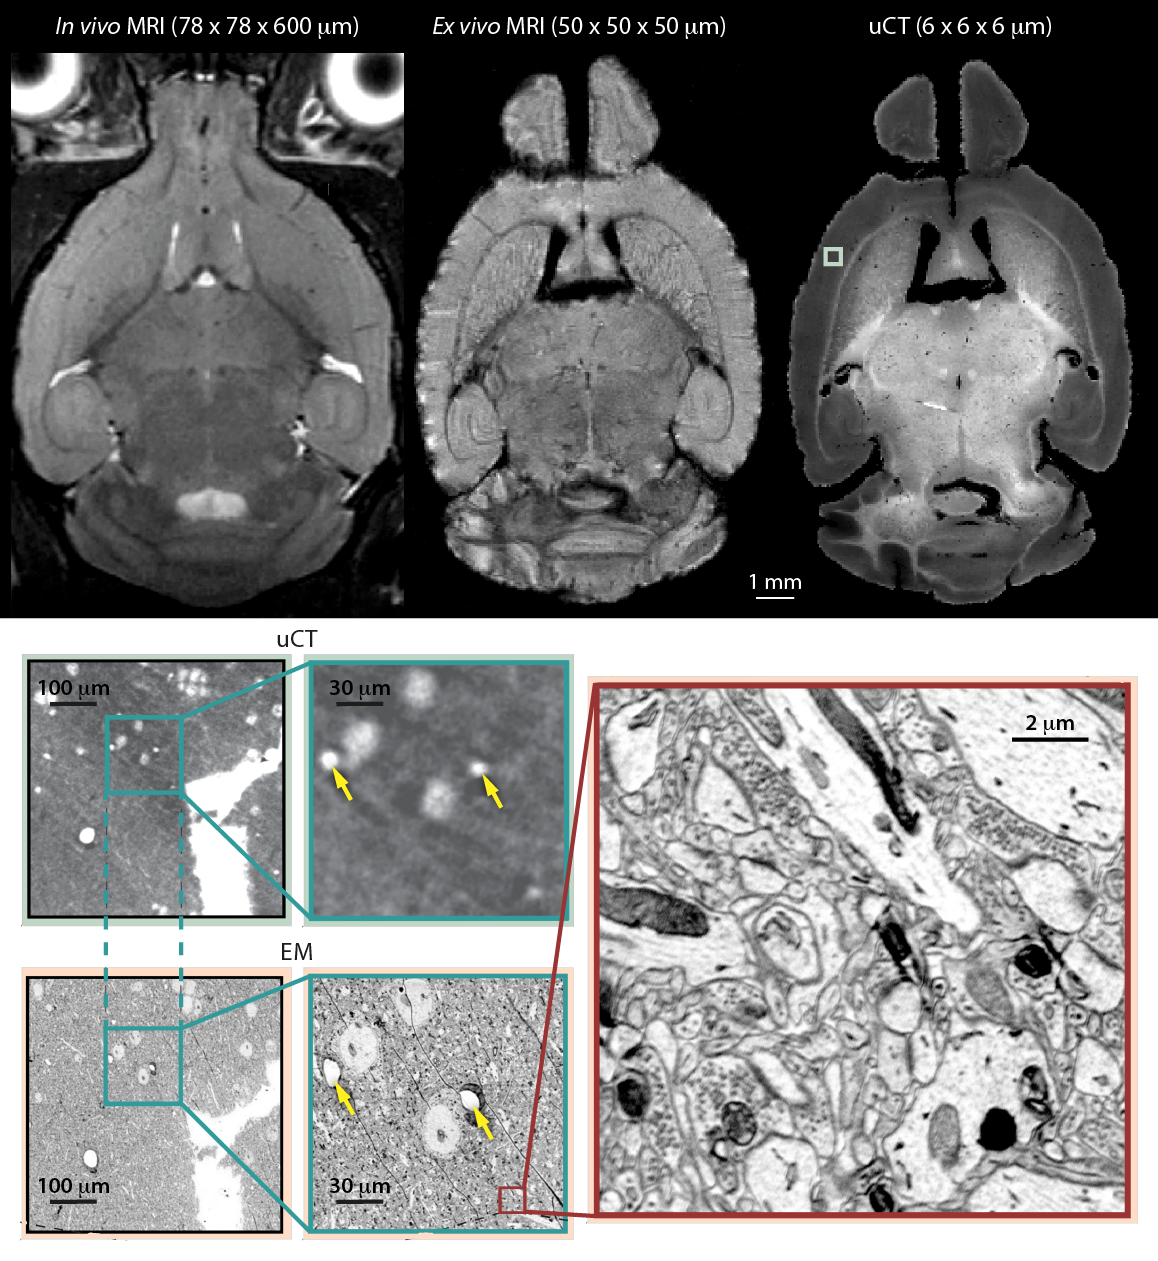
\includegraphics[width=7.5cm]{figs/grant_multi_scale}
  \end{figure}
\end{frame}

\begin{frame}
  \frametitle{Potential Aims}
  \textbf{The general scope of this project will be to develop and optimize a
    pipeline to use synchrotron x-ray \bolduct data to validate, characterize
    and compare diffusion MRI reconstruction and tractography
    algorithms.}\newline

  Potential Aims:
  \begin{enumerate}
    \item Optimize \uct data acquisition, pre-processing
    \item Use 3D structure tensor analysis to estimate ground truth ODFs from
      \uct data and perform quantitative comparisons with ODFs from MRI
    \item Use ODFs and segmented white matter tracts from the \uct data to
      evaluate MRI tractography algorithms
  \end{enumerate}
\end{frame}

\begin{frame}
  \frametitle{Aim 1: \bolduct data optimization}
  \begin{outline}
    \1 Specifics to be determined
    \1 Data acquisition ideas:

    \2 Characterize new detector hardware that is arriving soon
    \2 Accurately model and optimize acquisition to exploit x-ray phase contrast
    \2 Theoretical work on choosing beam energy to optimize CNR for metal stains
    
    \1 Data processing ideas:
    
    \2 Develop efficient computational pipeline to deal with massive data size
    \3 Full reconstruction on the order of 5-10 TB
    \3 Improve collaborators' current file size reduction methods
    \2 Addressing ring artifacts with post-processing algorithm\cite{Prell2009}
  \end{outline}
\end{frame}

\begin{frame}
  \frametitle{Ring artifacts example}
  \begin{center}
    \begin{tabular}[h]{c c}
      
\includegraphics[width=0.45\linewidth]{figs/bad_rings} & 
\includegraphics[width=0.45\linewidth]{figs/bad_rings_fixed} \\
      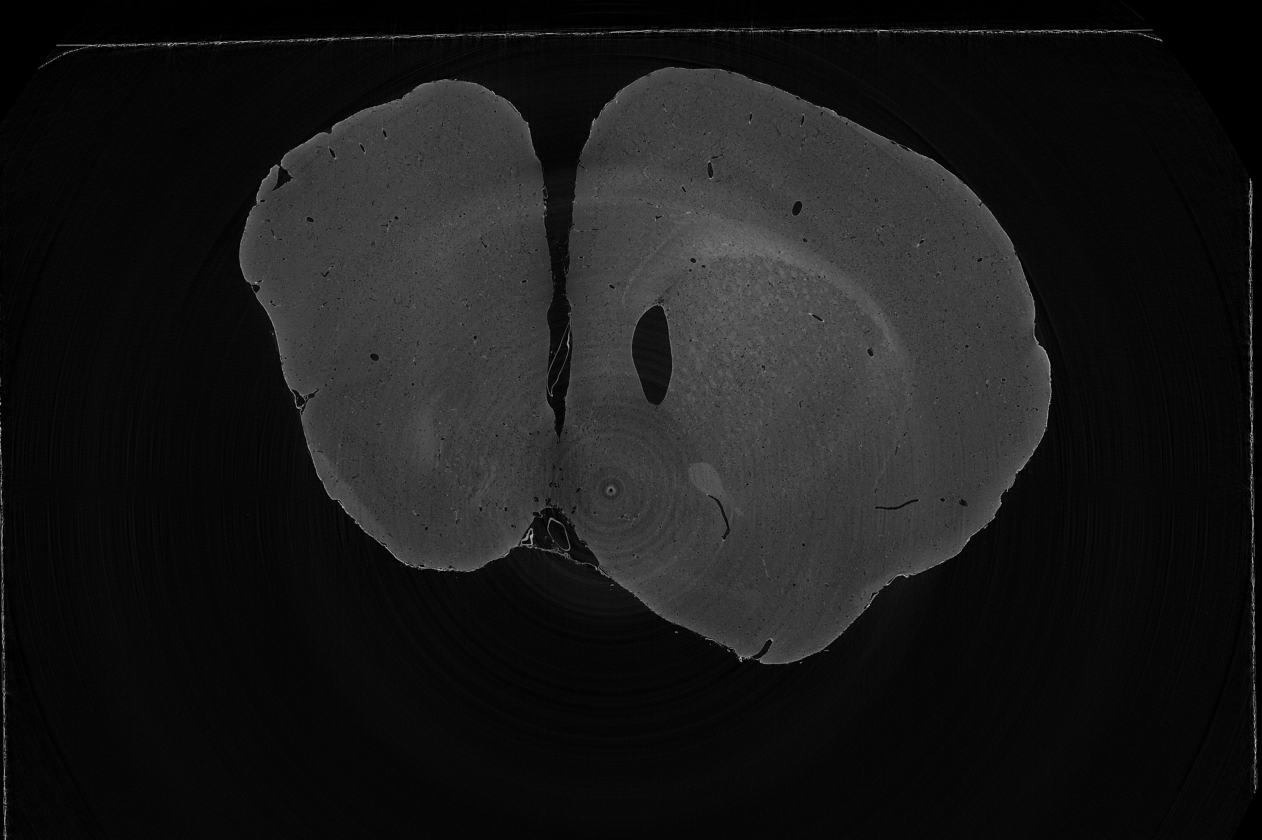
\includegraphics[width=0.45\linewidth]{figs/med_rings}  & 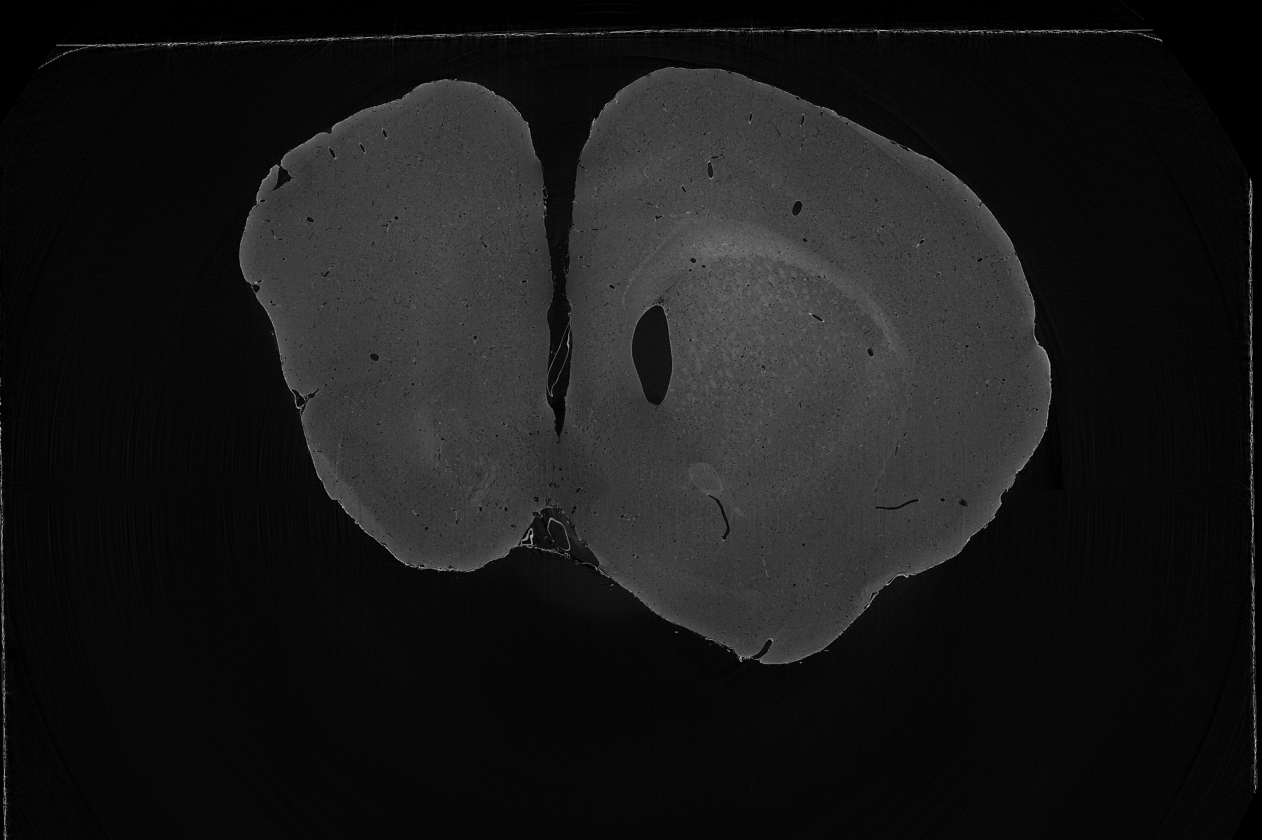
\includegraphics[width=0.45\linewidth]{figs/med_rings_fixed}
    \end{tabular}
  \end{center}

\end{frame}
\begin{frame}
  \frametitle{Aim 2: Validation of MRI ODFs with \bolduct using structure tensor
    analysis}
  Completed work:
  \begin{outline}
    \1 \uct ODF calculation pipeline is developed
    \1 \uct - MRI registration pipeline is developed and close to being implemented/validated
    \1 Preliminary ODF comparisons look promising
  \end{outline}
\end{frame}

\begin{frame}
  \frametitle{Aim 2: Preliminary results}
  \begin{center}
    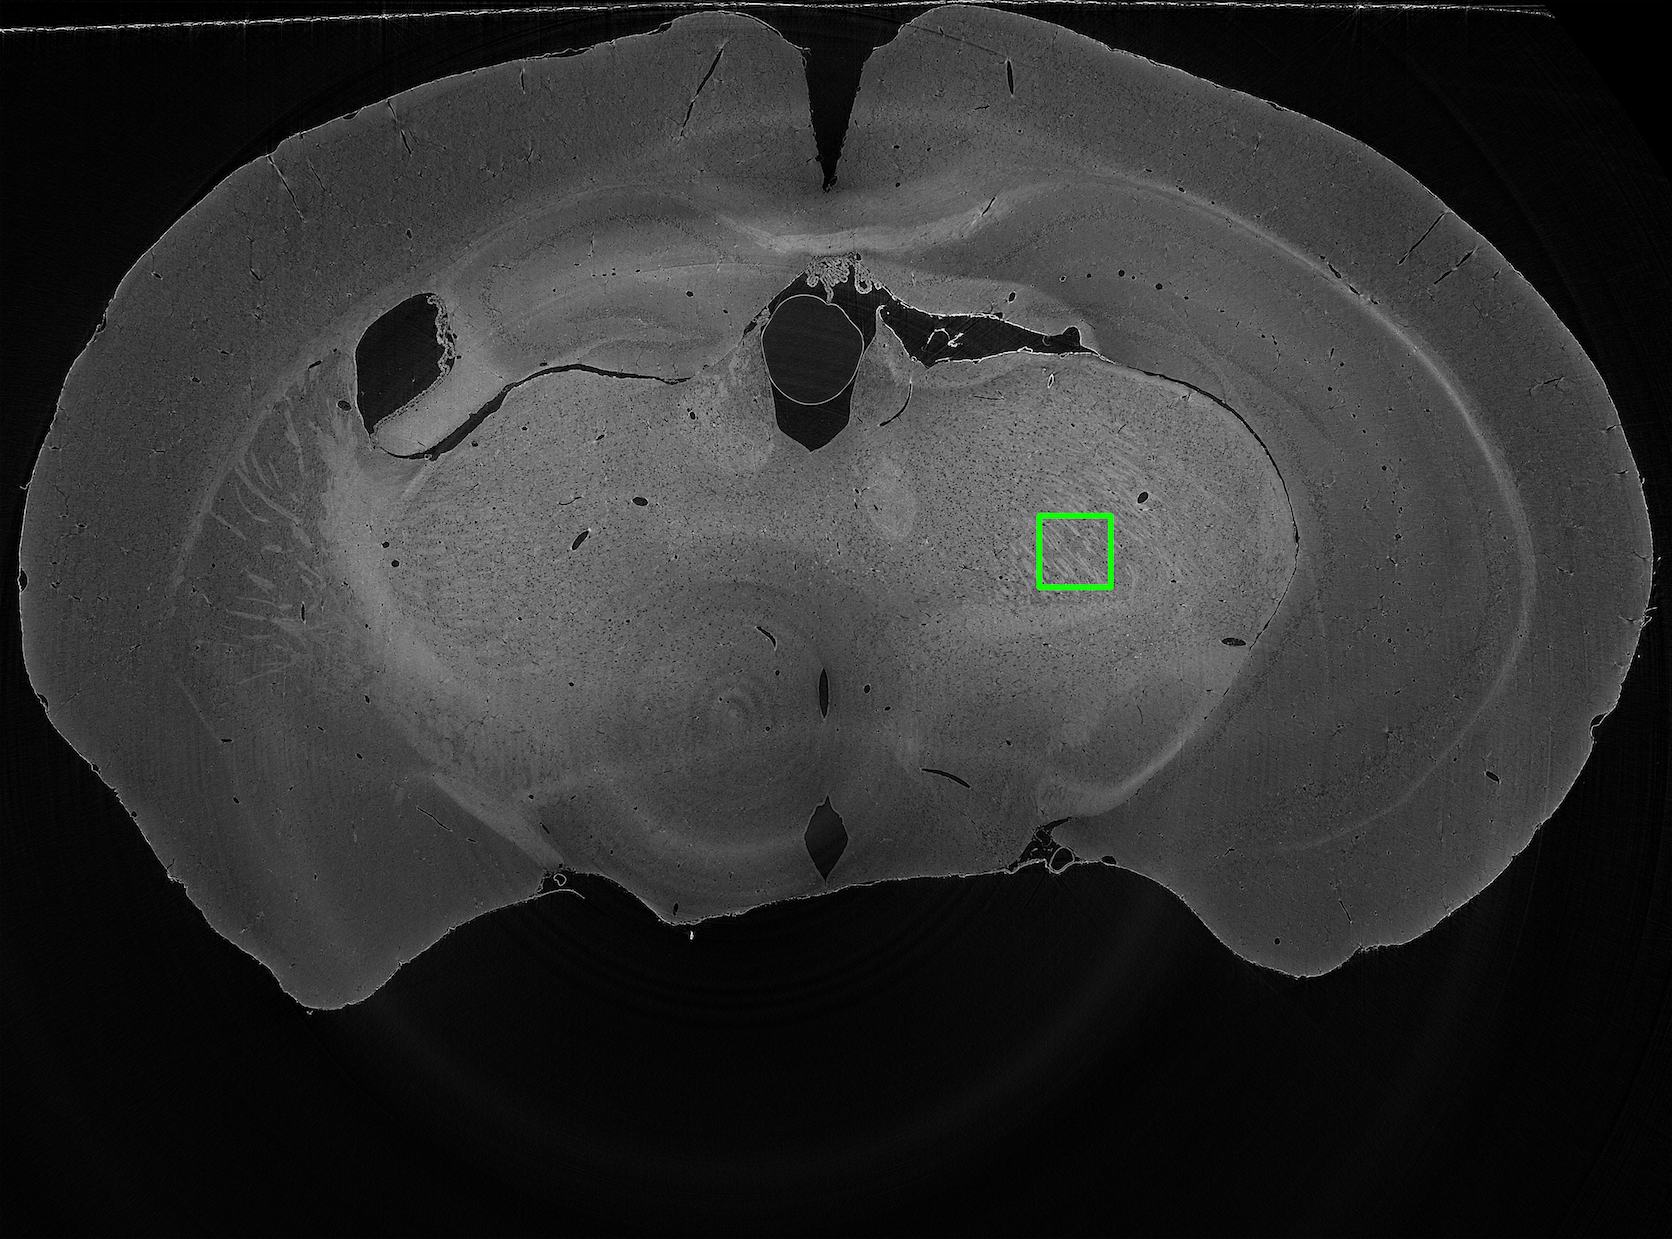
\includegraphics[width=0.95\linewidth]{figs/gordon_slice}
  \end{center}
  \begin{tikzpicture}[remember picture, overlay]
    \node[xshift=1cm, yshift=-1cm, anchor=north west] at (current page.north west){
      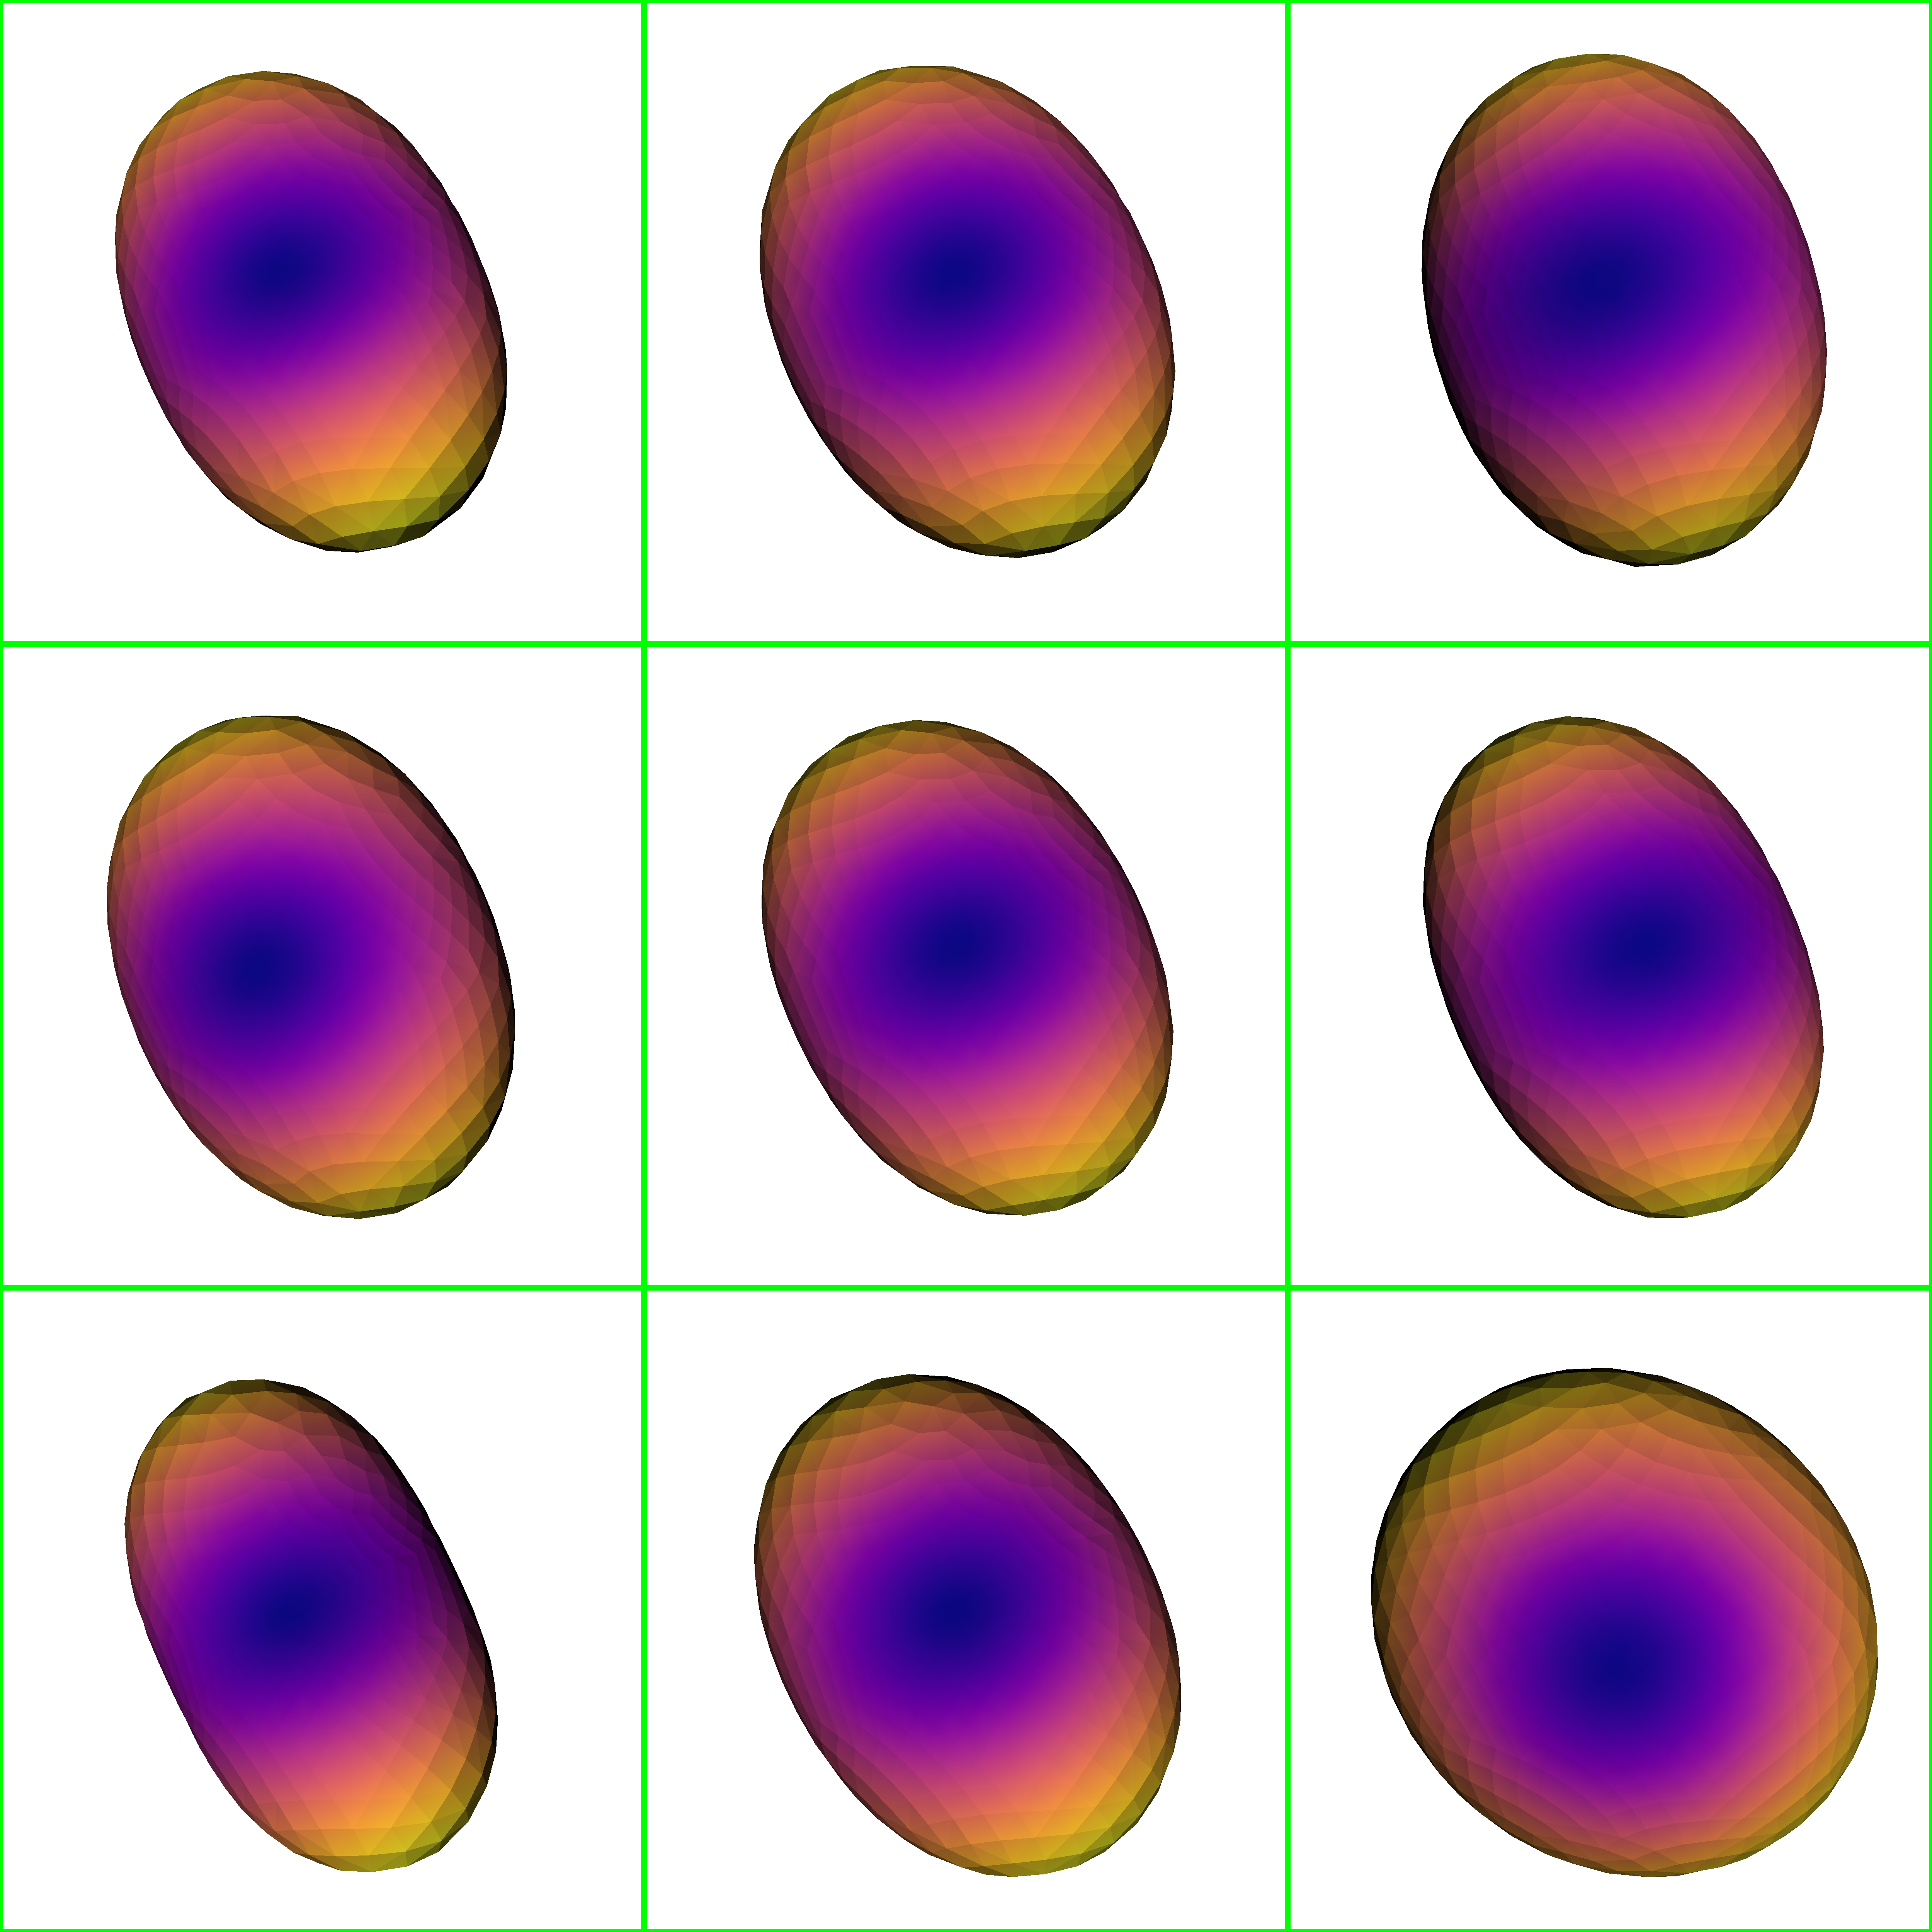
\includegraphics[width=3.75cm]{figs/gordon_DTI}
    };
    \node[xshift=1cm, yshift=-5cm, anchor=north west] at (current page.north west){
      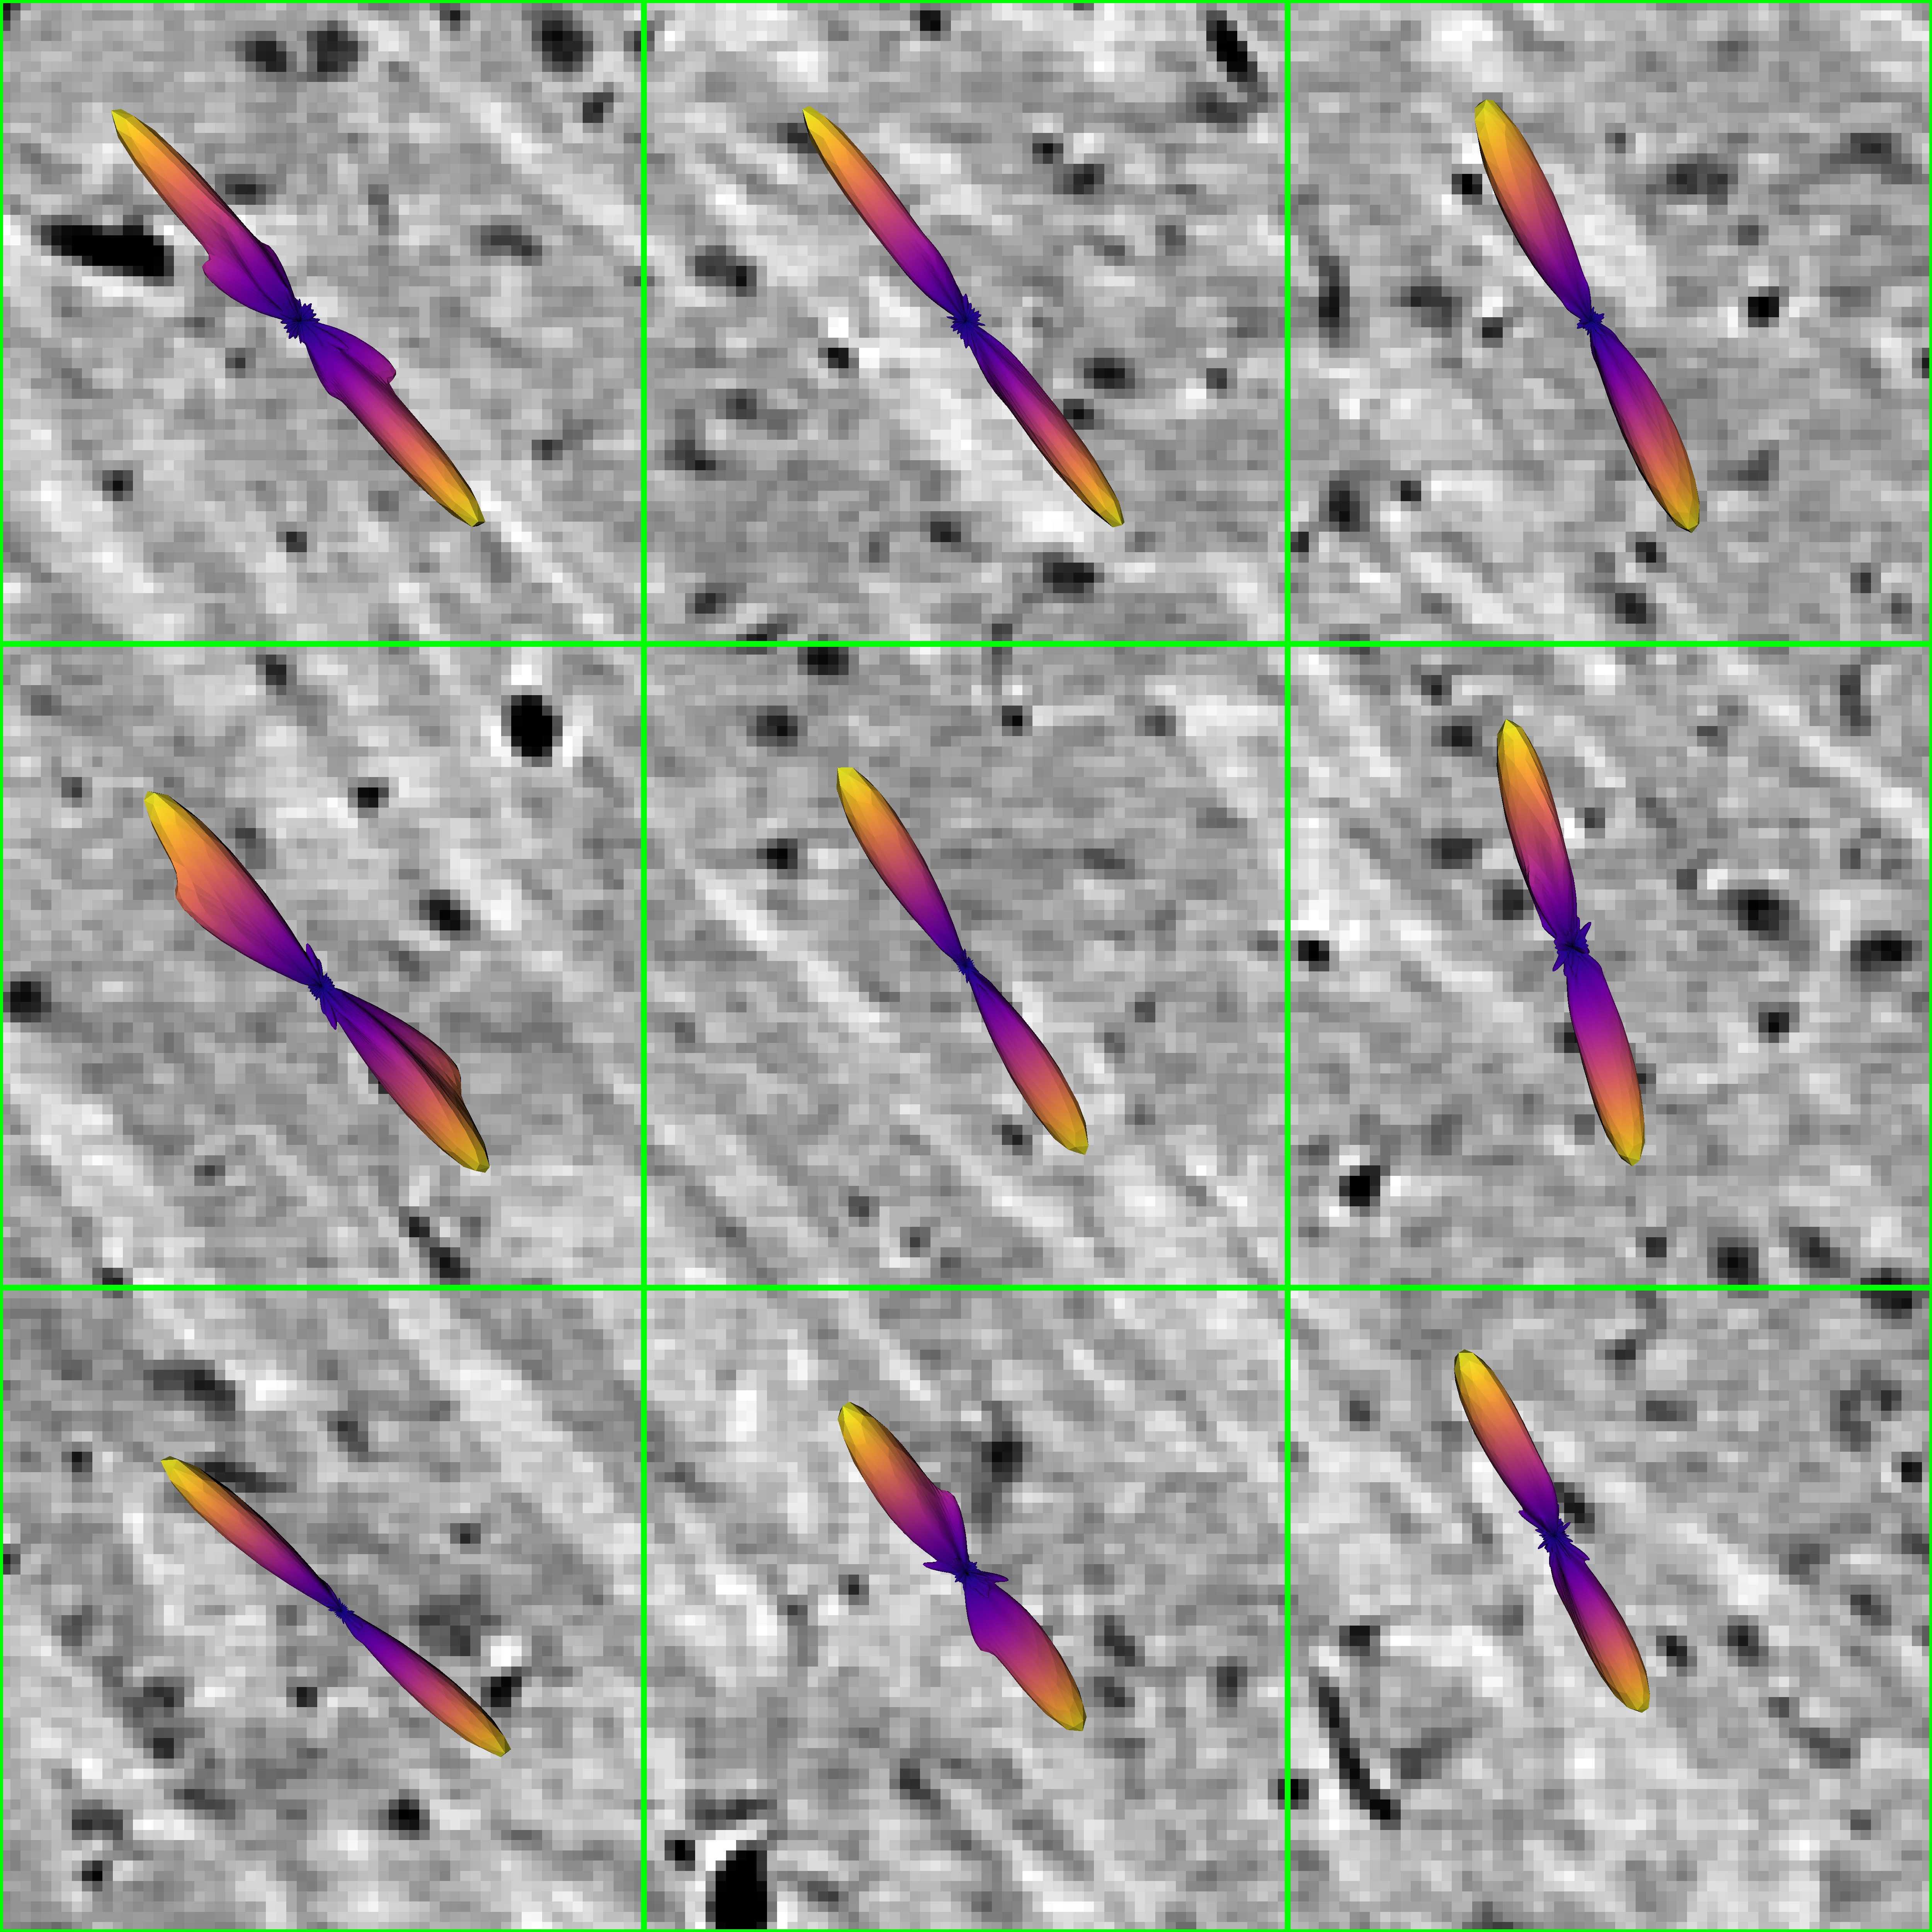
\includegraphics[width=3.75cm]{figs/gordon_uct}
    };   
  \end{tikzpicture}
\end{frame}

\begin{frame}
  \frametitle{Aim 2: Registration pipeline}
  Registrations are currently being computed with ANTs software from UPenn\cite{Avants2014, Klein2009}\newline

  Pipeline:
  \begin{enumerate}
  \item Calculate ODFs from full-res \uct data binned over ROI the size of a DW-MRI voxel
  \item Downsample \uct (\textapprox 1.2~\um) and structural MRI (\textapprox
    50~\um) to DW-MRI resolution (\textapprox 150~\um)
  \item Calculate linear and nonlinear diffeomorphic \cite{Avants2008} \uct $\rightarrow$ structural MRI transform
  \item Calculate linear structural MRI $\rightarrow$ DW-MRI transform
  \item Apply combined transforms to \uct ODFs
  \item Rotate \uct ODFs appropriately\cite{Alexander2001, Raffelt2012, Raffelt2011, Yap2011, Hong2009}
  \end{enumerate}
\end{frame}

\begin{frame}
  \frametitle{Aim 2: Registration pipeline}
  \begin{columns}
    \begin{column}{0.5\textwidth}
      \begin{center}
        \uct (green) $\rightarrow$ structural MRI (red)
        \vspace{1em}
        \includemedia[
        width=5cm,height=3.484848cm,
        activate=pageopen,
        addresource=figs/xray2struct.mp4,
        flashvars={
          source=figs/xray2struct.mp4
        }
        ]{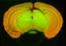
\includegraphics[width=5cm, height=3.484848cm]{figs/xray2structposter}}{VPlayer9.swf}        
      \end{center}
    \end{column}
    \begin{column}{0.5\textwidth}
      \begin{center}
        structural MRI (red) $\rightarrow$ DW-MRI (cyan)
        \vspace{1em}
        \includemedia[
        width=5cm,height=3.484848cm,
        activate=pageopen,
        addresource=figs/struct2dwi.mp4,
        flashvars={
          source=figs/struct2dwi.mp4
        }
        ]{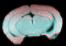
\includegraphics[width=5cm, height=3.484848cm]{figs/struct2dwiposter}}{VPlayer9.swf}                
      \end{center}
    \end{column}
  \end{columns}
\end{frame}

\begin{frame}
  \frametitle{Aim 2: Proposed work}
  \begin{outline}
  \1 Replicate other groups' histology results with \uct data
  \2 Use \uct ODFs over a large number of ROI as ground truth to compare
  performance of a number of DW-MRI reconstrucion models
  \2 Requires a new dataset with more directions for most HARDI algorithms

  \1 Characterize sensitivity / uncertainty with structure tensor method
  \2 Large number of tunable parameters that most groups do not adequately discuss

  \1 Potentially could get a spatial map of algorithm-specific DW-MRI reconstruction
  failure, characterize by tissue type, etc.
  \end{outline}
\end{frame}

\begin{frame}
  \frametitle{Aim 3: Tractography validation}
  Proposed work:
  \begin{outline}
    \1 Segment white matter tracts from \uct data
    \1 Compare to MRI tractography
    \1 Compare to tractograms generated from running MRI tractography algorithms on
    \uct ODFs from Aim 2
    \2 Eliminates registration error
    \2 Characterize tractography algorithm performance with many free parameters:
    \3 Can calculate ODFs at arbitrary ``voxel size''
    \3 Can calculate ODFs using different models (fit to tensor instead of SH)
  \end{outline}
\end{frame}

\begin{frame}
  \frametitle{Segmentation vs. tractography}
  \begin{columns}
    \begin{column}{0.5\textwidth}
      \begin{center}
        \uct segmentation
        \includemedia[
        width=5.5cm,height=3.4178cm,
        activate=pageopen,
        addresource=figs/3d_movie.mp4,
        flashvars={
          source=figs/3d_movie.mp4
        }
        ]{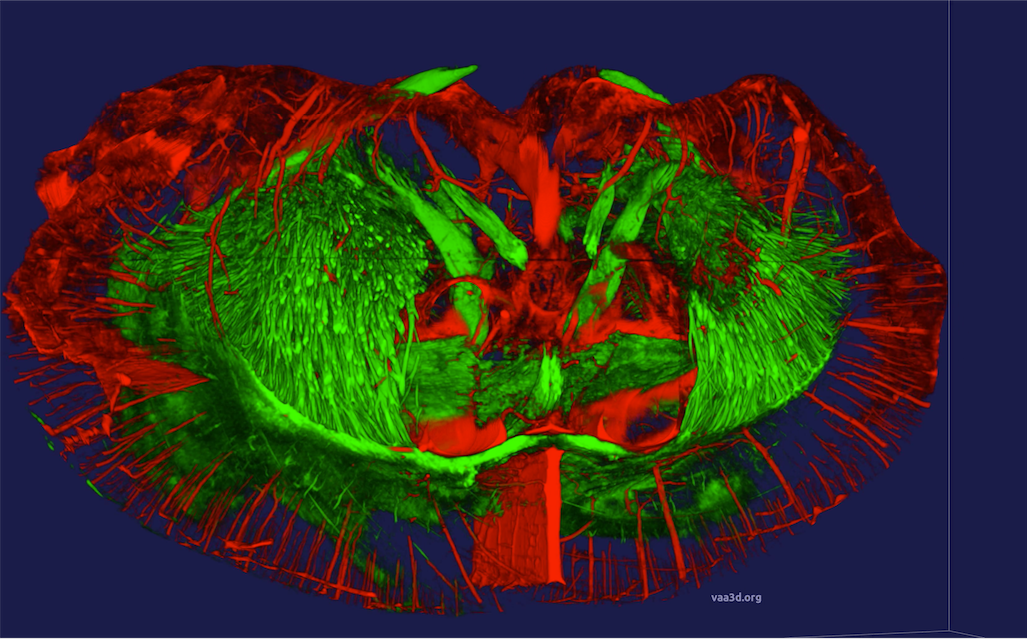
\includegraphics[width=5.5cm, height=3.4178cm]{figs/3d_movieposter}}{VPlayer9.swf}        
      \end{center}
    \end{column}
    \begin{column}{0.5\textwidth}
      \begin{center}
        DW-MRI tractography
        \includemedia[
        width=5.5cm,height=4.2246cm,
        activate=pageopen,
        addresource=figs/TRACTOGRAPHY_ROT.mp4,
        flashvars={
          source=figs/TRACTOGRAPHY_ROT.mp4
        }
        ]{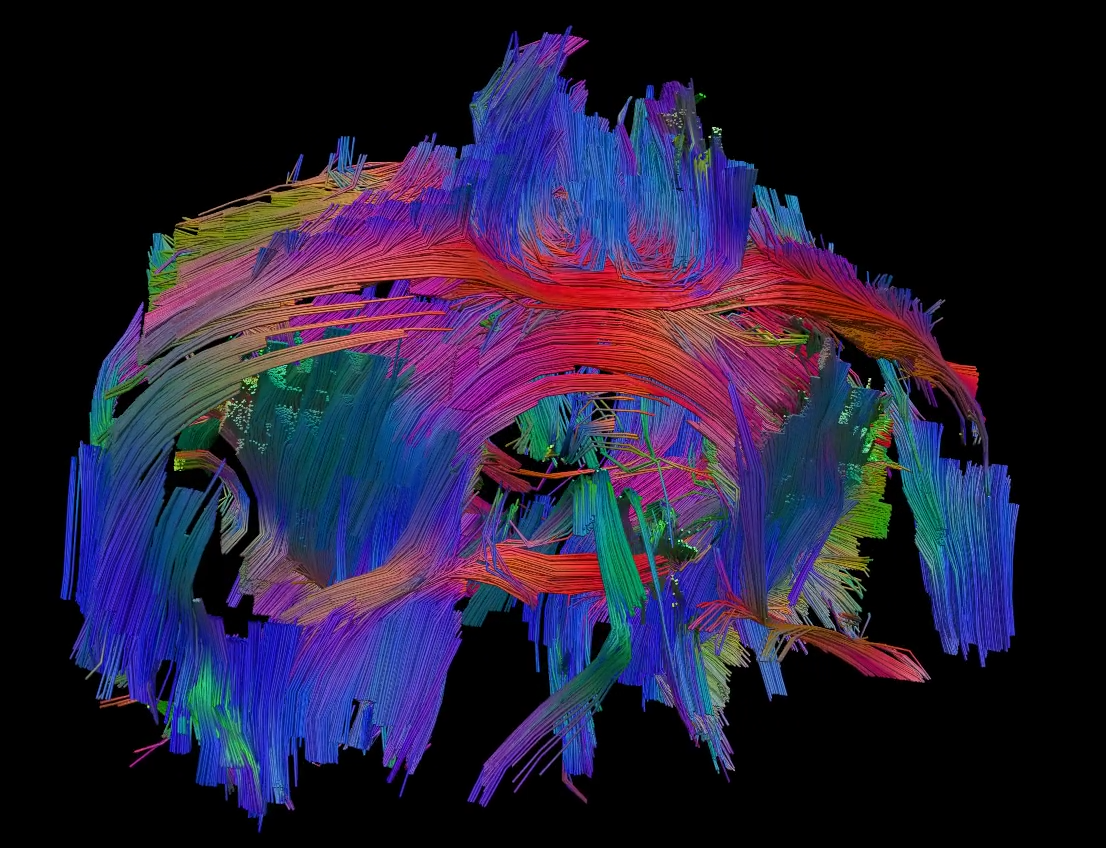
\includegraphics[width=5.5cm, height=4.2246cm]{figs/TRACTOGRAPHY_ROTposter}}{VPlayer9.swf}                
      \end{center}
    \end{column}
  \end{columns}  
\end{frame}

\begin{frame}
  \frametitle{Graduation timeline}
  \begin{outline}
    \1 December 8, 2018 - submit F31 grant proposal
    \1 Winter quarter 2019 - complete GPMP thesis proposal
    \1 Spring 2021 - graduation 
  \end{outline}
\end{frame}

\begin{frame}[allowframebreaks]
  \frametitle{References}
  \printbibliography
\end{frame}

\begin{frame}
  \frametitle{\bolduct ODFs: phantom validation}
  \begin{columns}
    \begin{column}{0.48\textwidth}
      \begin{center}
        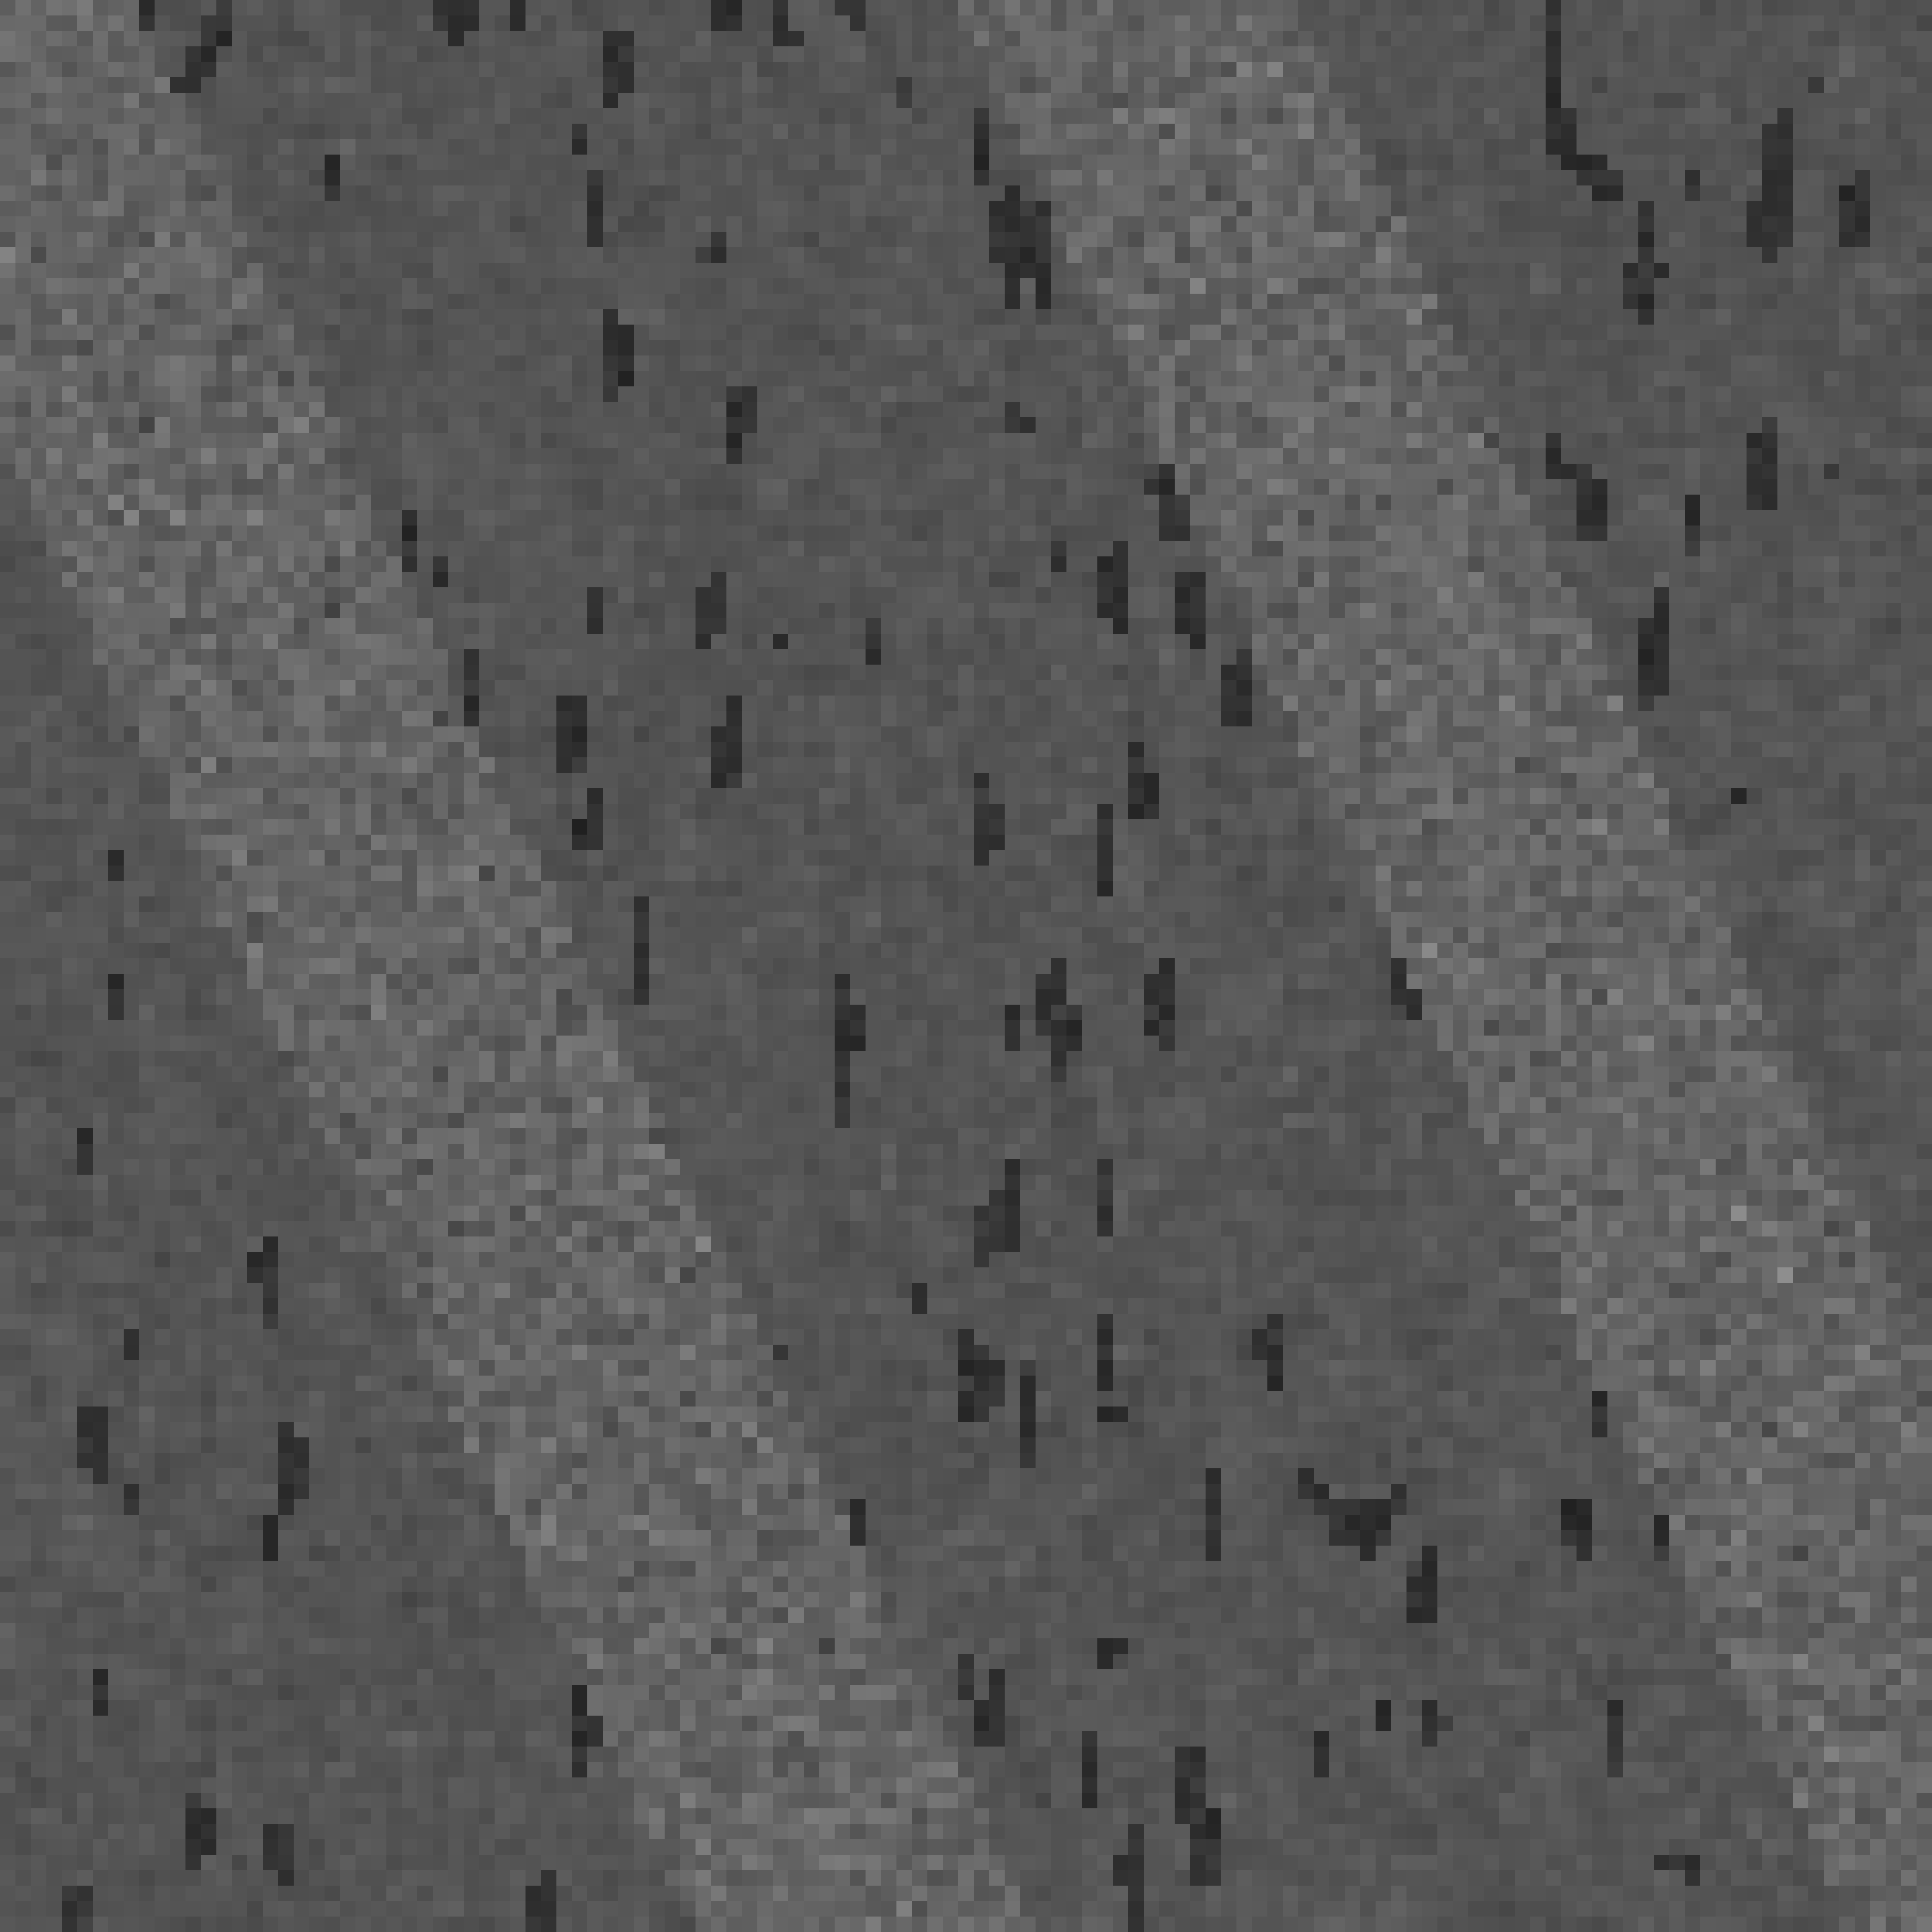
\includegraphics[height=0.42\textheight]{figs/phant25_angle}
        \vspace{4em}
        \scalebox{-1}[1]{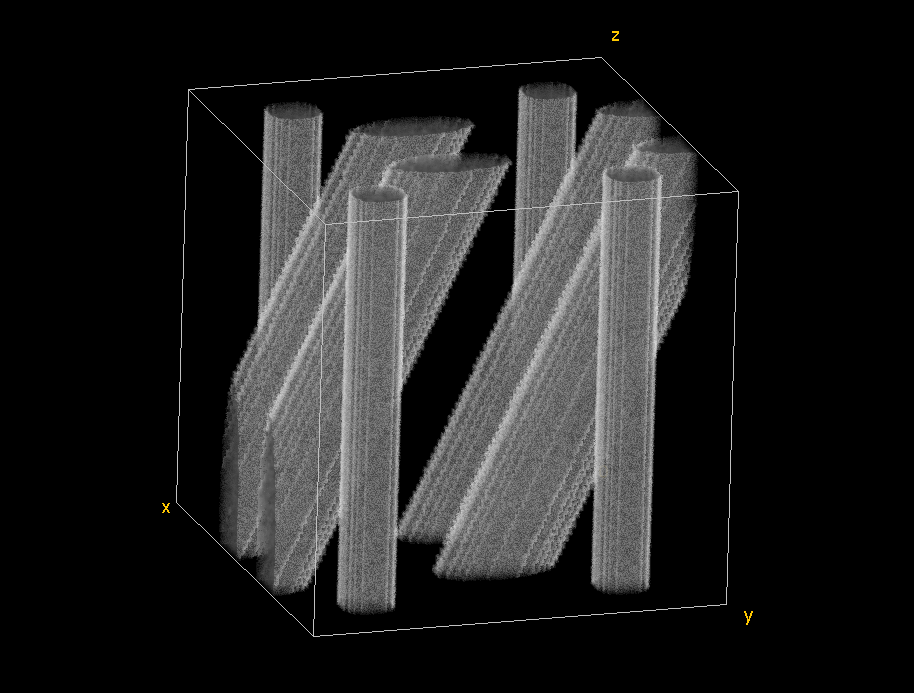
\includegraphics[height=0.42\textheight]{figs/phantom_volume}}
      \end{center}
    \end{column}
    \begin{column}{0.48\textwidth}
      \begin{center}
        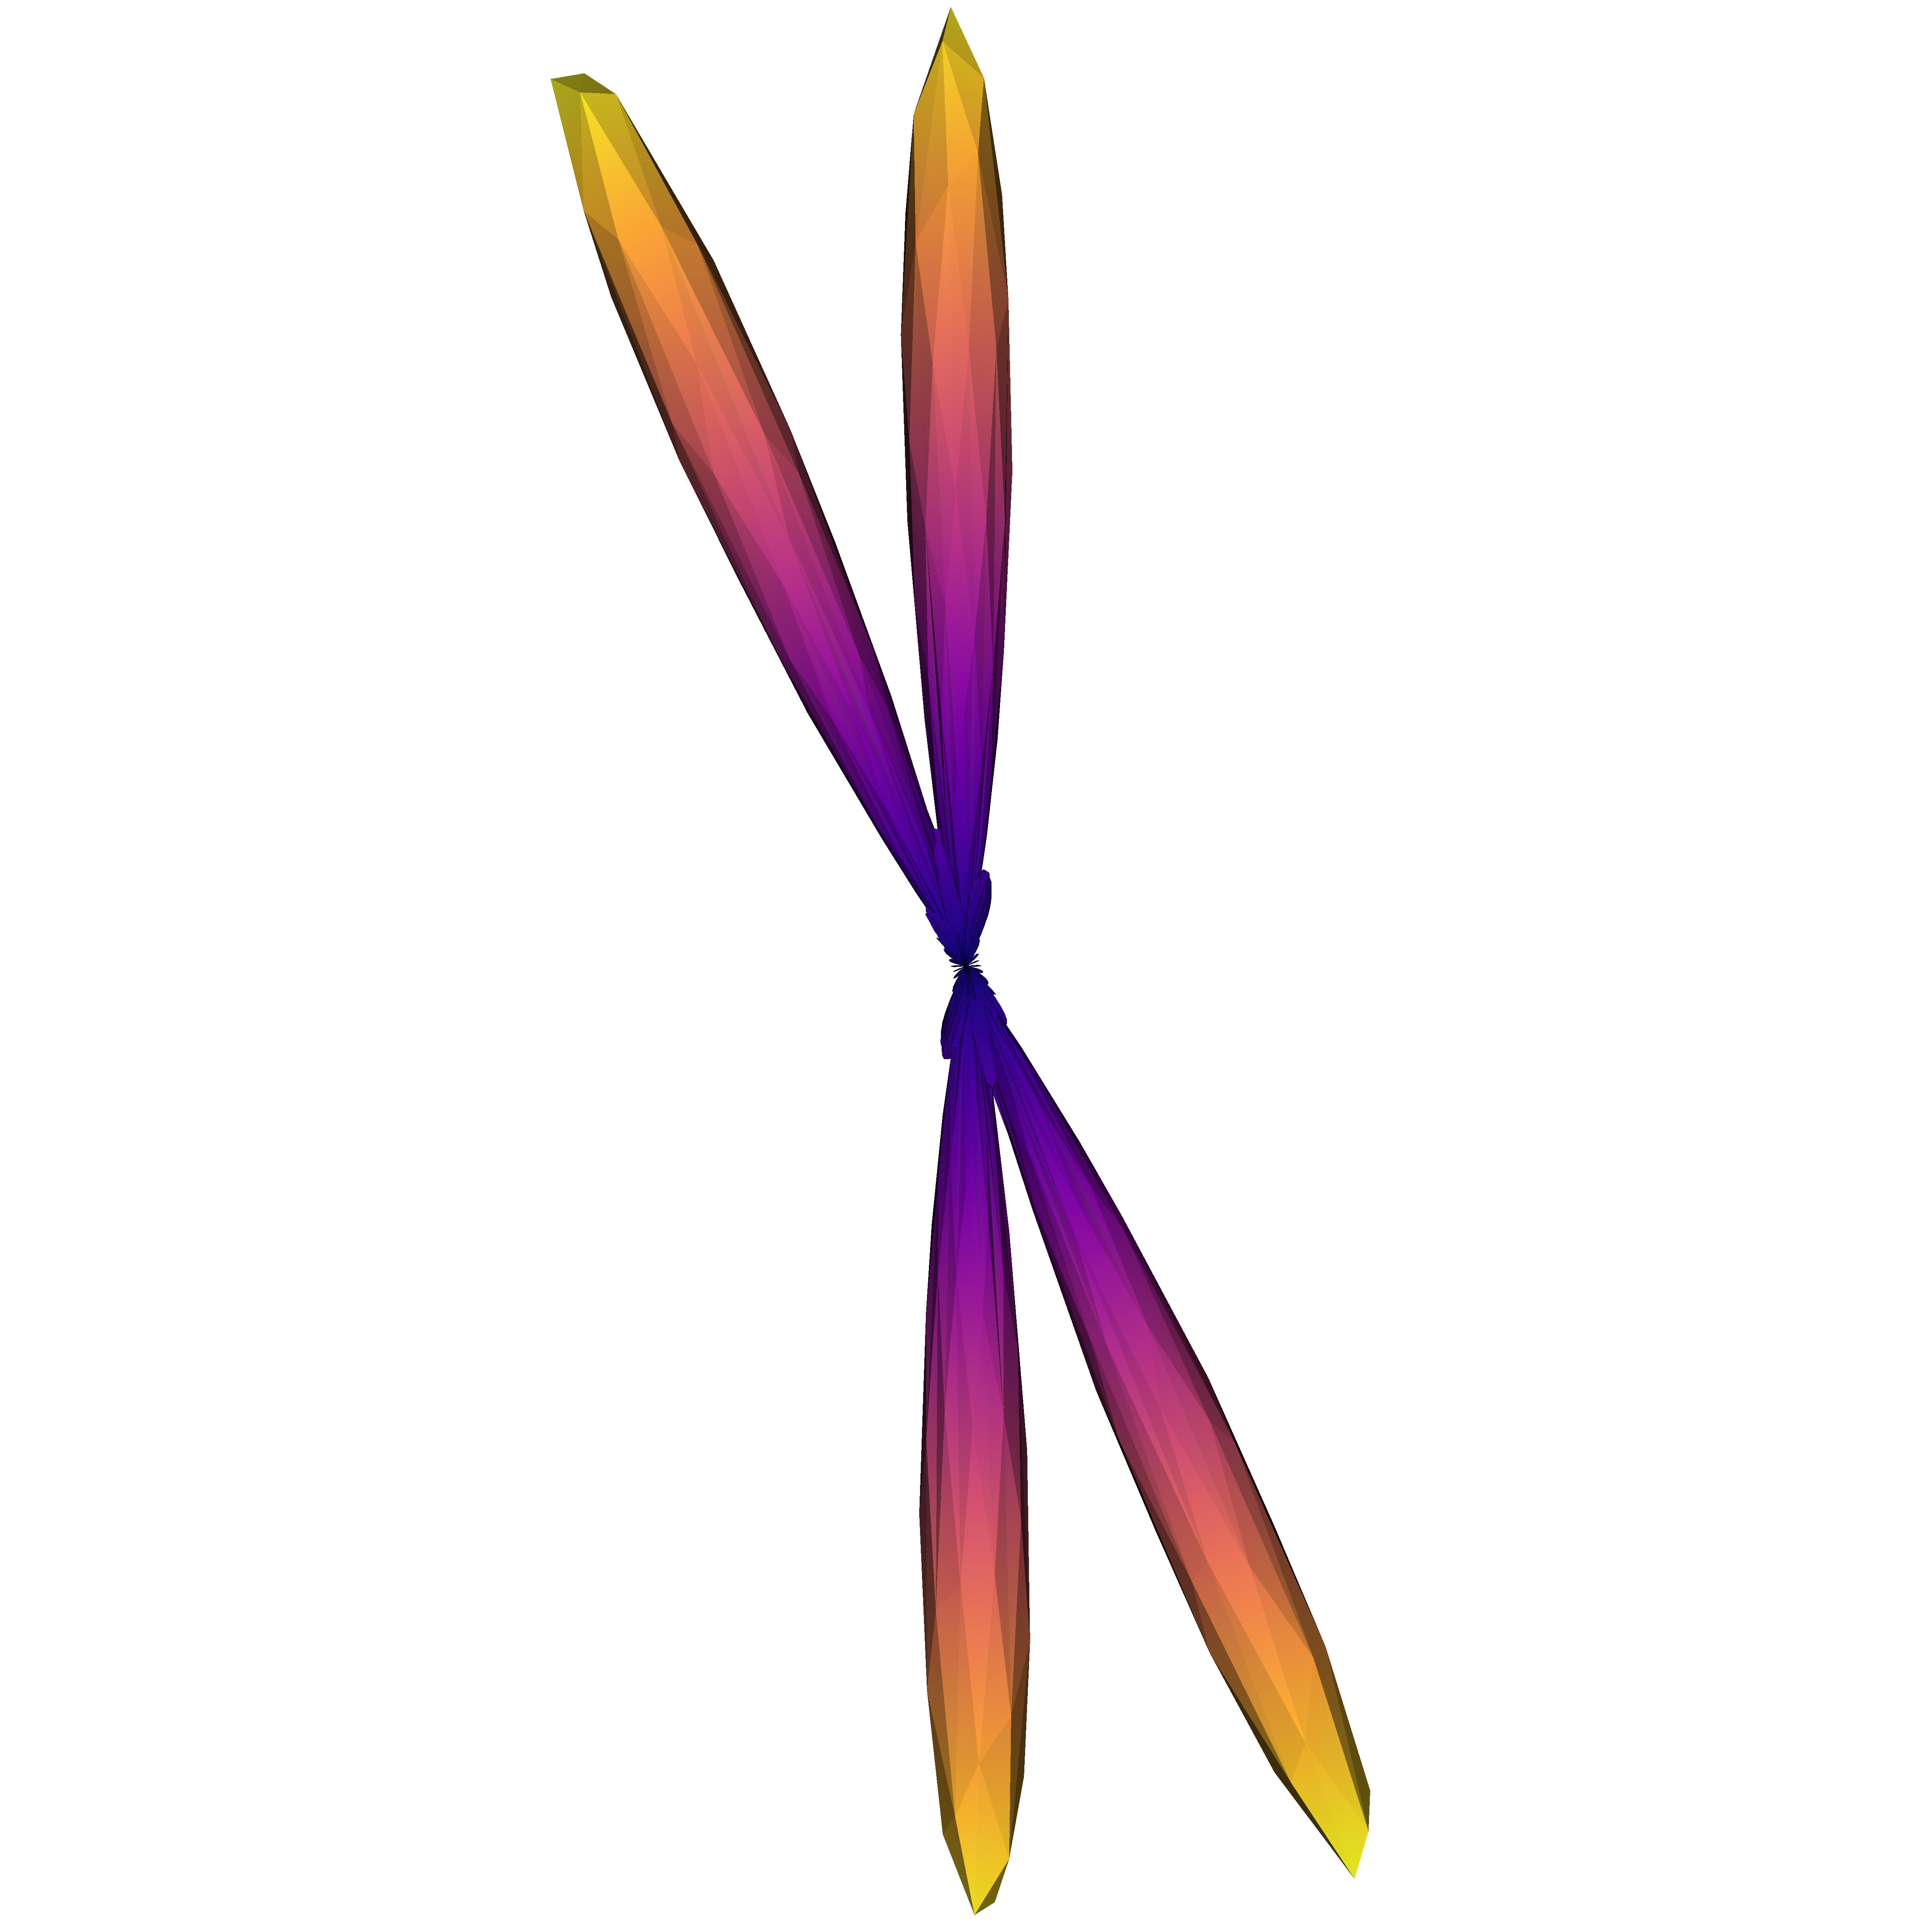
\includegraphics[width=\linewidth]{figs/phant_25_ST_ODF}
      \end{center}      
    \end{column}
  \end{columns}
\end{frame}

\begin{frame}
  \frametitle{Structure tensor analysis}
  \vspace{1em}
  For a 3D intensity image $f(x,y,z)$, with gradient
  $\nabla f = (f_x, f_y, f_z)$:
  \begin{align}
    \text{ST}\left(f\right)(x,y,z) &= g_{\sigma_N} \circledast
    \begin{pmatrix}
      f_x^2 & f_x f_y & f_x f_z \\
      f_x f_y & f_y^2 & f_y f_z \\
      f_x f_z & f_y f_z & f_z^2 \\
    \end{pmatrix}
    \nonumber
  \end{align}
  The eigenvector with the smallest eigenvalue is an estimate of local fiber
  orientation. In an ROI containing $K$ such fiber orientation vectors, the ODF
  can be written in spherical coordinates:
  \begin{align}
    \text{ODF}(\theta, \phi) = \frac{1}{K}\sum_{k=1}^K \delta(\theta - \theta_k)\delta(\phi - \phi_k)\nonumber
  \end{align}
  The ODF can be expanded on the real spherical harmonics, $Y_l^m(\theta, \phi)$, up to degree $L_{max}$:
  \begin{align}
    \hat{\text{ODF}}(\theta, \phi) &= \sum_{l=0}^{L_{max}}\sum_{m=-l}^l c_{lm}Y_l^m(\theta, \phi)\nonumber\\
  \end{align}
\end{frame}
\end{document}